\documentclass[letterpaper, 10 pt, conference]{ieeeconf}  % Comment this line out
                                                          % if you need a4paper
%\documentclass[a4paper, 10pt, conference]{ieeeconf}      % Use this line for a4
                                                          % paper

\IEEEoverridecommandlockouts                              % This command is only
                                                          % needed if you want to
                                                          % use the \thanks command
\overrideIEEEmargins
% See the \addtolength command later in the file to balance the column lengths
% on the last page of the document

\usepackage[utf8]{inputenc}
\usepackage[T1]{fontenc}
\usepackage{graphicx}
\usepackage{float}
\overrideIEEEmargins

\title{Project Proposal}
\author{Patrick Armstrong, Ryan Williamson, Caleb Edwards}
\date{February 2020}

\begin{document}

\maketitle

\begin{abstract}
    
\end{abstract}

\section{Introduction and Motivation}
For our project we want to build a smart sprinkler controller based off of different weather sensors placed throughout a user's yard. A zone is a subsystem in a sprinkler system that is controlled from a valve box. There are multiple zones controlled by one valve box. The goal of this project is to provide real time feedback to the user to make informed decisions on when and for how long to water each zone. 

As of now, a person with a sprinkler controller has to go to their sprinkler box in their garage and manually enter times and duration for each zone in their yard. Not many people are sure how long or what time of day they should even water their yard. It is almost an educated guess for most people with controllers. Based off of these times and duration settings that are manually entered, the old controller will turn on and water that zone for the specified duration. We would like to make the controller smarter. 

Our system will be based on recommendations. There will be sensors that collect data throughout the day and get stored in our controller. Based on these results, a predictive algorithm that we will create will send a recommendation to the UI stating a duration and time that the user should water that zone. The user will then be able to accept these recommendations, stick with the default settings, or enter some manual settings based on their preference. 

There are endless possibilities with a sprinkler controller and the data that could be collected from different weather sensors. Our controller will collect data from a hub station that will represent a weather station. This will allow the user to also have that extra functionality on their system, viewed through the UI. So if a user would like to base their input to the controller based on these results, they can do so. Each zone of the sprinkler system will have different sensors, including a moisture sensor placed in the dirt of that zone. The data fed to the controller from these results are how the recommendations are determined for unique times of each zone. 

\begin{figure}[H]
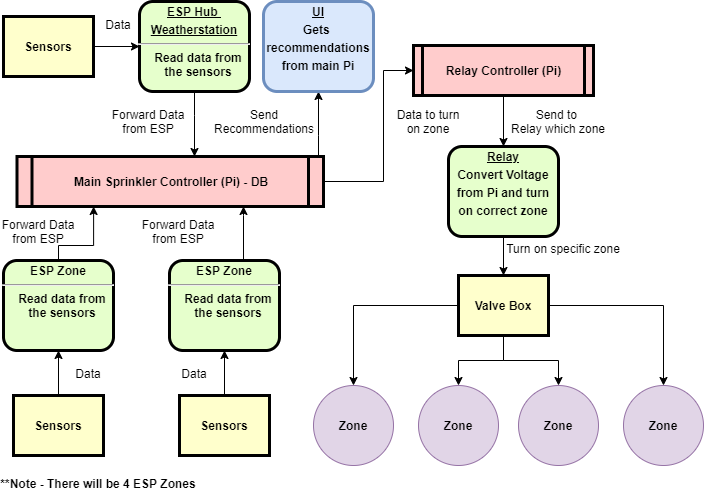
\includegraphics[scale=.4]{Diagram.png}
\caption{Block Diagram of Sprinkler Controller}
\end{figure}

\section{Project Tasks and Specific Task Interfaces}
There will be many different tasks involved in the creation of a smart sprinkler system. Below we will specify the different tasks needed for this project, including their difficulty and if the necessity of having them.

\subsection{Communication Between ESP and Sensors}

\subsection{Communication Between ESP and Raspberry PI}

\subsection{User Interface}

\subsection{Data Storage}

\subsection{Predictive Algorithm}

\subsection{Relay to Turn on Zones}

\section{Testing and Integration Strategy}
\subsection{Individual Testing}
Testing will be done with distinct and unique portions of the project. Every portion of the project that can be ran without integration will be tested separately, before integrating. Data being read from each sensor to an ESP will be tested separate from the rest of the project until we know we can integrate. The communication from the ESP to the PI will be done separate with small test data. This will allow us to know we get the communication correct, before we move on to integration. 

There will be testing on turning on the valve using a Pi. This portion of testing will be to make sure that a Pi with a relay can turn on the valve for a sprinkler system. 

\subsection{Integration Testing}
Once we have data from the sensors being read by the ESP, and valid communication from the Pi and the ESP; we will be able to integrate these tasks into data being read from the ESP and transferred to the Pi. This will then allow for testing on the predictive algorithm. Once we have data onto the Pi, we can test the algorithm to see if we have results that make sense from the data that we are actually reading. 

\section{Group Management and Communication Plan}
Our group communication plan consists of two different platforms. We will use Discord for real time, fast communication. We will use Github for the management of all tasks and document storage. 

Discord will be for all of our immediate communication. If we have a time pressing question that needs to be discussed, Discord allows real time communication. Discord also allows file sharing if the team needs to view something in that exact moment. 

Github will allow us to all have access to our repository, as well as view the project plan and tasks associated with this repo. The project portion of Github allows you to use a Kanban style management for the agile project management. This process will allow us to view the progress of each other to see if we are falling behind in different areas. This will allow us to manage our time and help others with certain tasks if we realize we are falling behind. 

\section{Schedule and Milestones}

\section{Risk Assessment}
\subsection{UI}

\subsection{Wireless Communication?}

\section{Bill of Materials}

\section{Vendor List}

\section{Conclusion}

\begin{thebibliography}{99}
\bibitem{c1} % Add rest of citation here
\end{thebibliography}

\end{document}
